\section*{Sources of Preference Measures: Alliance Portfolios and UN Voting}

Given that we cannot directly observe state preferences, scholars have attempted to estimate preferences using two main behavioral indicators: who states choose to ally with and how states vote at the United Nations (UN). The idea behind alliance portfolio measures is that we can infer a state's foreign policy by looking at the states they choose to align with. In the extreme case, if two states have all of the same allies, it is likely that their foreign policy goals are quite similar. Conversely, if all allies of one state are not allied to another, and vice versa, our best guess is that these states would have different aims and desires in foreign policy. \citet{buenodemesquita:lalman:2008} encapsulate the logic when they note that ``alliance commitments reflect a nation's position on major international issues''. Measures of alliance behavior do, however, suffer from the fact that these measures are largely static and sparsely occurring. Formal alliances are relatively constant over time, whereas in many cases state preferences will be more fluid, and therefore these scores will be at best a lagging indicator of preferences. Furthermore, as \citet{hage:2011} points out, the fact that links are so rare creates an artificial similarity of alliance portfolios.

We also have a relatively large corpus of behavioral information in UN Voting Records. The cost of voting in the UN is low, and so, scholars have argued that measures of affinity based on UN voting are relatively representative of the underlying distribution of preferences \citep{gartzke:1998}. This is especially fortuitous because the methodology of inferring preferences from voting in a legislature is relatively advanced. A few issues with these measures are that the potential benefit of winning UN votes is low, and so states might have incentives to vote against their preference as they are not costly signals, and the distribution of UN voting is prone to large supermajorities of the type rarely seen in ``ordinary" legislatures.

\subsection*{Current measures of preferences: S-Scores}

 The initial measure used to measure preference similarity based on alliance portfolios was Kendall's $\tau_{B}$ \citep{buenodemesquita:lalman:2008}. This measure is:
 
 \begin{equation}
	 \tau_{B} = \frac{n_{c} - n_{d}}{\sqrt{(n_{0} - n_{1})(n_{0} - n_{2})}}
 \end{equation}
 
 \noindent where $n_{c}$ is the number of pairs where both actor $i$ and $j$ have the same rank ordering (for example both the United Kingdom and the United States are more closely allied to Israel than to Iran), $n_{d}$ is the number of pairs where they have discordant rankings (the United States is more closely allied to Saudi Arabia than to Russia, Syria is more closely allied to Russia than to Saudi Arabia). The denominator attempts to adjust the total number of pairs with the number of ties: $n_{0}$ is the total number of pairs ($n(n-1)/2$), $n_{1}, n_{2}$ are measures for ties in both $i$ and $j$'s rankings respectively.
 
\citet{signorino:ritter:1999} convincingly pointed to flaws in this measure, notably its focus on rank-ordering as applied to a context where we instead care mostly about the presence or absence of an alliance. In addition, if we add additional strategically irrelevant states, we will create artificially high $\tau_{B}$ statistics. Thus, Signorino and Ritter introduce the S-score, which has since been the most widely used alliance similarity measure.\footnote{\citet{bennett:rupert:2003} also find a stronger relationship between theoretical predictions and results when using S-scores than when using $\tau_{B}$.} The equation for the S-score is:

\begin{equation}
	S(P^i, P^j, W, L) = 1 - 2w_k \frac{d(P^i, P^j, W, L)}{d^{\text{max}}(W,L)}
\end{equation}

\noindent where $d(P^i, P^j, W, L) = \sum_{k = 1}^N \frac{w_k}{\Delta^\text{max}_{k}} |p^i_k - p^j_k|$. In $d(P^i, P^j, W, L)$, $w_k$ is the $k$'th element of a weight matrix, $d^\text{max}(W,L)$ is the maximal distance on a given dimension, and $\Delta$ is a normalizing constant. For the weight matrix, generally, analysts have used S-scores calculated with a weight matrix of ones--giving each potential ally equal weight--though the other plausible choice would be to weight states by importance, for example using their share of world military capability, as calculated by \citet{singer:small:1995}. \citet{gartzke:1998} attempted to apply a similar S-score methodology to UN voting data and created the ``Affinity of Nations'' index. An important point for these scores is that they are purely dyadic. One can look at the S-score between two states, but one cannot look at a state's preferences in comparison to a larger cluster, or note the movement in a states preferences over time. In monadic analysis, these score measures are not even available, and once we are dealing with situations involving more than two states, the number of S-scores necessary to fully characterize the preferences balloons quickly (it is the number of actors choose two). 

An advantage of utilizing UN General Assembly Voting, is that it allowed the field to take advantage of methodological advances that have been made in the study of legislatures \citep{poole:rosenthal:1985}. \citet{bailey:etal:2015} do so by using an Item Response Theory model on UNGA voting. This model seeks to place states on a unidimensional latent preference space using their voting behavior. The assumption of this model is that states' votes on a resolution are a function of states' ideal points, characteristics of the vote, and random error. In particular, for each bill $v$, a state's vote will be based on the latent variable $Z_{itv}$:

\begin{equation}
	Z_{itv} = \beta_{iv}\theta_{it} + \epsilon_{iv}
\end{equation}

\noindent such that the state will vote yes if $Z_{itv} < \gamma_{1v}$, no if $Z_{itv} > \gamma_{2v}$ and otherwise abstain. Here, $\theta_{it}$ is state $i$'s ideal point at time $t$, and $\beta_{iv}$ is the discrimination parameter of a particular bill $v$. When $\beta_{v}$ is positive, states with high ideal points will be more likely to vote no. When it is negative, they will be more likely to vote yes.

The authors specifically fix the parameters $\gamma_{1v}$ and $\gamma_{2v}$ such that the same bill will have the same value in different years, and they standardize and normalize $\theta$. They also use $\theta_{it-1}$ as a prior on $\theta{it}$. With these constraints, they solve for the ideal points using a Metropolis Hastings Markov Chain Monte Carlo (MCMC).

Both methods relying on UN data, and those relying on alliances have difficulties distinguishing within '0's and '1's. For example, if we know two states are allies, we have reason to believe they have similar preferences, but if we know they are not allies, it is not clear whether they are enemies or they are indifferent -- the United States is ``not-allies" with both Bhutan and North Korea for example. As of 2012, using the Correlates of War projects alliance data, only about 1/8th of all dyads were between countries with any sort of alliance. Similarly, with UN voting, so many UN votes contain super-majorities and states vote together a huge proportion of the time. If we only look at yes and no votes in the UN general assembly, the median pair of states has voted together about 96\% of the time. If we include abstentions,  they have voted together 86\% of the time. So when two states vote together it is hard to distinguish between states voting together because of similar preferences, or just preferences that are not radically dissimilar. Both S-scores and Item Response theory succeed in adding granularity and nuance to these rough measures, but they are both limited by focusing only on a relationship between two states. 

We can see the potential issues of focusing only on direct relations when we view how these two measures of preference treat relations over the Korean peninsula. If we take China, North Korea, South Korea, and the United States, we would expect the United States and South Korea to have preferences that are similar to each other and dissimilar from China and North Korea (and vice versa). Yet, if we look at extant measures of preferences (as of 2012), as depicted in Figure \ref{korean:prefs}, they do not seem to effectively characterize this relationship. S-scores based on alliance portfolios posit that China and the two Koreas are closely clustered, with the United States distant from all three, while ideal point distances put South Korea as equidistant between the United States and North Korea. Now it could be that these measures are producing a novel, counterintuitive, result, but given the failures of extant preference measures to add much to our predictive models of conflict, one might be skeptical.

\begin{figure}[ht]
	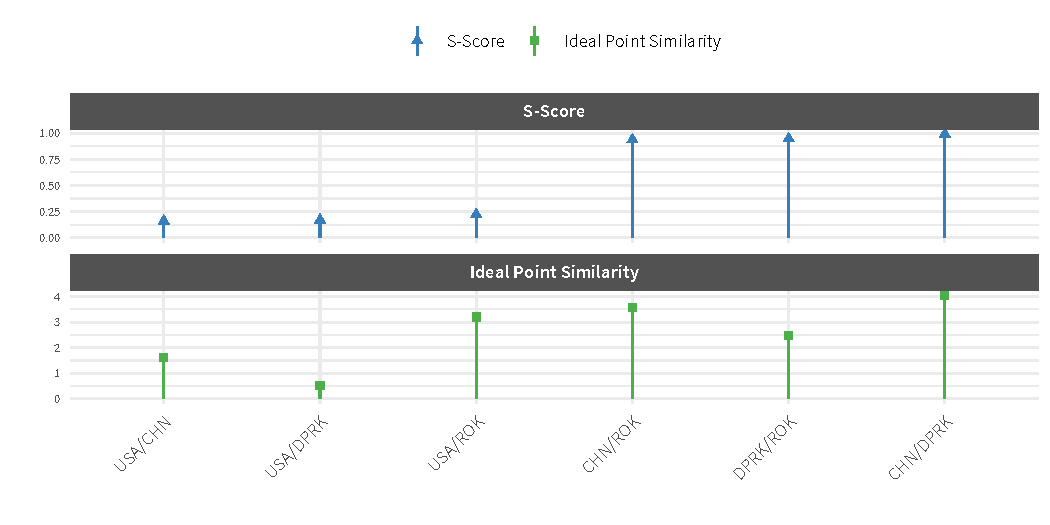
\includegraphics[width=1\textwidth]{idPtScoreViz.pdf}
	\caption{Visualization of ideal point distance and S-score relationships between China (CHN), North Korea (DPRK), South Korea (ROK), and the United States (USA) in 2012. We have rescaled each of these measures to be between 0 and 1 for comparability, where a 1 indicates that states are farther apart and a 0 that states are closer together.}
	\label{korean:prefs}
\end{figure}

The sources of these surprising results become more clear when looking at the data on which they are based. In 2012, according to the Correlates of War, North Korea only had 3 alliances -- a non-aggression pact with the South, and alliances with Russia and China. Similarly, South Korea's only alliances were that non-aggression pact, and an alliance with the United States. Given the United States' many other allies, there was much more divergence between their alliance portfolio and South Korea's, than there was between the two Koreas' portfolios \citep{gibler:sarkees:2004}. Similarly, when looking at voting patterns at the UN, South Korea voted 50\% of the time with the US, 63\% of the time with North Korea, and 70\% of the time with China.

Even using this data, we can better approximate state preferences when we treat alliances and UN voting as relational data. When it comes to alliance behavior, the fact that North Korea was allies with China and Russia, and South Korea with the United States could give us additional information, because the alliance behaviors of countries such as the United States and China are so divergent. When looking at voting patterns at the UN, the data is even more unexpected. In 2012, South Korea voted 50\% of the time with the US, 63\% of the time with North Korea, and 70\% of the time with China.

We thus argue that two changes can substantially improve our measures of state preferences. First, both alliances and UN voting contain information about state foreign policy preferences, and given the limits of this information, we should find a way to use both. Second, by using network techniques and treating this data as relational data, we can wring more information from the stone, and get both a more nuanced, and more accurate view of state affinity and state preferences.